\documentclass[tikz,dvisvgm,border=0pt]{standalone}
% Shared preamble of the diagrams in vignettes/articles/cuda-kernels.Rmd.
% Render them with `make diagrams` from the package root.
\usepackage[T1]{fontenc}
\usepackage{lmodern}
\usepackage{tikz}
\usetikzlibrary{arrows.meta, positioning, fit, backgrounds, calc, shapes.geometric, decorations.pathreplacing}

\definecolor{host}{HTML}{3B6EA8}
\definecolor{device}{HTML}{2E8B57}
\definecolor{accent}{HTML}{C0571B}
\definecolor{muted}{HTML}{6B6B6B}

% A white card behind every figure, so that it reads in pkgdown's dark mode.
\tikzset{
  every picture/.append style={
    show background rectangle,
    background rectangle/.style={fill=white, rounded corners=6pt},
    inner frame sep=8pt,
    font=\sffamily\small,
    >={Stealth[length=2.2mm]},
  },
  box/.style={draw, rounded corners=3pt, thick, align=center, inner sep=5pt, fill=white},
  hostbox/.style={box, draw=host, fill=host!8},
  devbox/.style={box, draw=device, fill=device!8},
  accbox/.style={box, draw=accent, fill=accent!8},
  region/.style={draw=#1, rounded corners=6pt, thick, dashed, inner sep=8pt},
  heading/.style={font=\sffamily\bfseries\small, text=#1},
  note/.style={font=\sffamily\footnotesize, text=muted, align=center},
  flow/.style={->, thick},
  code/.style={font=\ttfamily\footnotesize},
}

\begin{document}
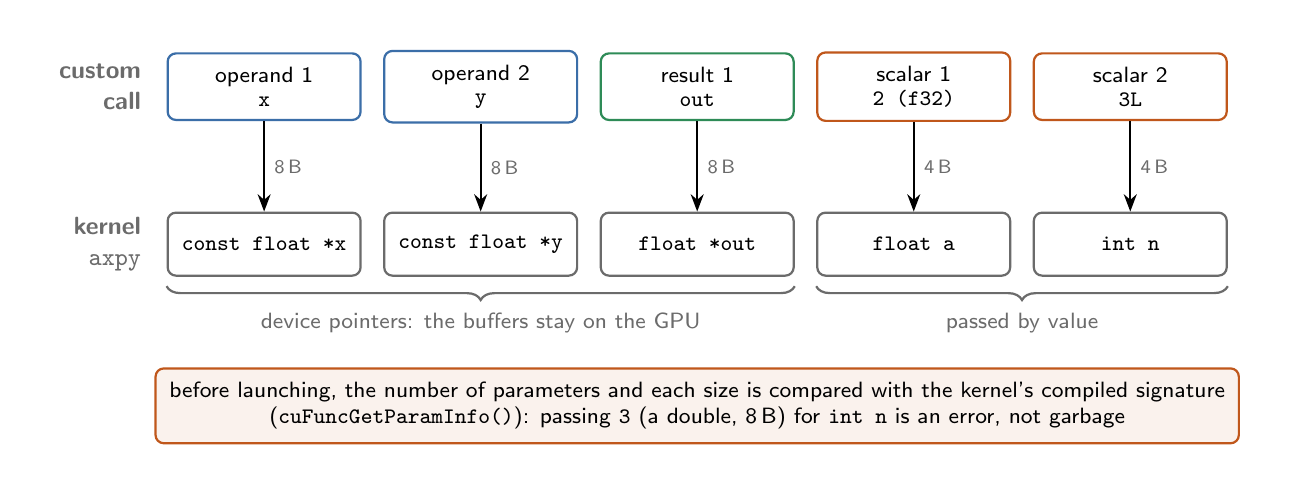
\begin{tikzpicture}[
    slot/.style={box, minimum width=2.45cm, minimum height=0.8cm, font=\ttfamily\footnotesize},
    size/.style={font=\sffamily\scriptsize, text=muted},
  ]
  \def\dx{2.75}
  % what the custom call provides
  \node[hostbox, slot] (a0) at (0, 0) {{\sffamily operand 1}\\[-1pt]x};
  \node[hostbox, slot] (a1) at (\dx, 0) {{\sffamily operand 2}\\[-1pt]y};
  \node[devbox, slot] (a2) at (2*\dx, 0) {{\sffamily result 1}\\[-1pt]out};
  \node[accbox, slot] (a3) at (3*\dx, 0) {{\sffamily scalar 1}\\[-1pt]2 (f32)};
  \node[accbox, slot] (a4) at (4*\dx, 0) {{\sffamily scalar 2}\\[-1pt]3L};
  \node[heading=muted, anchor=east, align=right] at ($(a0.west) + (-0.2, 0)$) {custom\\call};

  % what the kernel declares
  \foreach \t/\k in {{const float *x}/0, {const float *y}/1, {float *out}/2, {float a}/3, {int n}/4} {
    \node[box, slot, draw=muted] (p\k) at (\k*\dx, -2.0) {\t};
  }
  \node[heading=muted, anchor=east, align=right] at ($(p0.west) + (-0.2, 0)$) {kernel\\\texttt{axpy}};

  \foreach \k/\b in {0/8, 1/8, 2/8, 3/4, 4/4} {
    \draw[flow] (a\k) -- node[right, size] {\b\,B} (p\k);
  }

  \draw[decorate, decoration={brace, amplitude=5pt, mirror}, thick, muted]
    ($(p0.south west) + (0, -0.12)$) -- ($(p2.south east) + (0, -0.12)$)
    node[midway, below=6pt, note] {device pointers: the buffers stay on the GPU};
  \draw[decorate, decoration={brace, amplitude=5pt, mirror}, thick, muted]
    ($(p3.south west) + (0, -0.12)$) -- ($(p4.south east) + (0, -0.12)$)
    node[midway, below=6pt, note] {passed by value};

  \node[accbox, anchor=north, font=\sffamily\footnotesize, align=center] at ($(p2.south) + (0, -1.15)$)
    {before launching, the number of parameters and each size is compared with the kernel's compiled signature\\
     (\texttt{cuFuncGetParamInfo()}): passing \texttt{3} (a double, 8\,B) for \texttt{int n} is an error, not garbage};
\end{tikzpicture}
\end{document}
